\begin{figure}[htbp]
\centering
\begin{tikzpicture}[x=1cm,y=1cm]
\node[anchor=south west,inner sep=0] at (0,0) {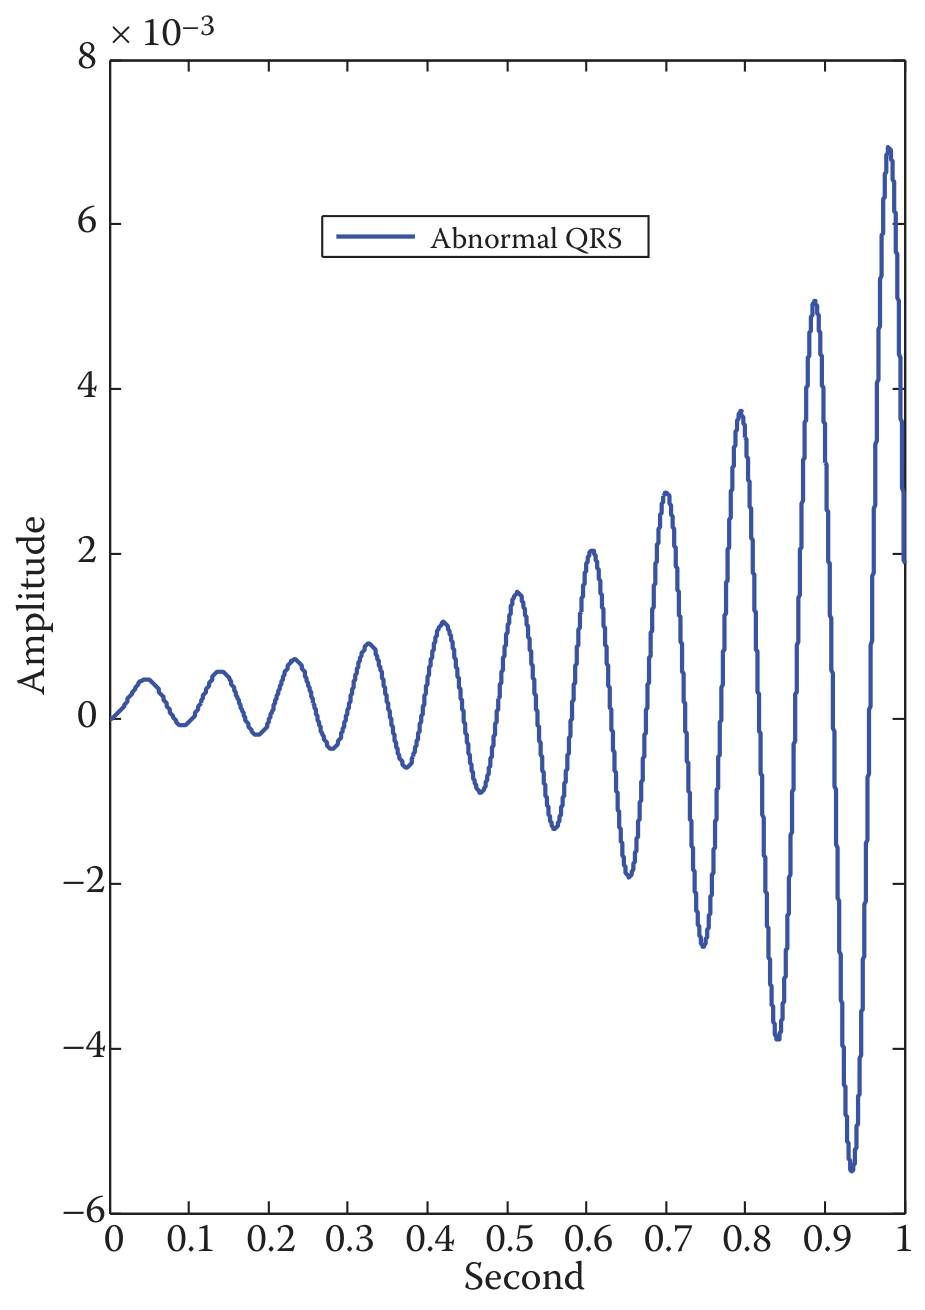
\includegraphics[width=9.0cm]{figures/ch03_fig08_data.png}};
\fill[white] (4.1692,10.2795) rectangle (6.2757,10.6103);
\fill[white] (4.4824,0.0841) rectangle (5.7239,0.5219);
\node[font=\scriptsize,rotate=0,inner sep=0] at (5.1031,0.3030) {时间（秒）};
\fill[white] (0.1067,5.9560) rectangle (0.5542,7.7501);
\node[font=\scriptsize,rotate=90,inner sep=0] at (0.3304,6.8530) {振幅};
\node[font=\scriptsize,rotate=0,inner sep=0] at (5.1206,10.4108) {异常 QRS};
\end{tikzpicture}
\origfig{8}{异常 QRS 波群所对应心脏系统的单位冲激响应曲线。}
\label{fig:ch03-08}
\end{figure}
